The detailed description for classes are the following:

\begin{enumerate}
    \item \textbf{Perfect Match}. This label is assigned when utterance has only 1 sense, and it is fully transferred with an image. If image could not transfer fully the sense of utterance and it could be done only with context knowledge, then also this label is assigned. There should be no factual mistakes, image should not be specific to cultural differences. The heuristic rule was to question yourself "Could i possibly came to this phrase, knowing image and context?". 
    \item \textbf{Partial Match}. This label is assigned when utterance has 2 or more distinct senses and image transfers one of them fully. It also should not be specific to culture or contain mistakes. In fact rules are the same as for Perfect Match, but applied to one of the senses in the utterances contains 2 or more senses.
    \item \textbf{Undefined}. This label is assigned when image is specific to cultural differences or when image can not transfer one of the senses of the utterance and the context could not help to recover untransferred sense.
    \item \textbf{No Match}. This label is assigned when image contains factual errors about utterance or when none of the entities from utterance present in the image.
\end{enumerate}

\smallskip

A decision tree was designed as the primary instruction for the labeling process, which aimed to assist the assessors in assigning appropriate labels to the samples. The decision tree was presented in Figure~\ref{LabelingMethod} and consisted of closed questions at each node, or terminal nodes containing the desired label. The assessors were instructed to follow the decision tree, starting from the root node and answering the questions until the label for each sample was reached. This strategy yielded high inter-rater reliability among the 3 assessors, indicating its efficacy in achieving consistent labeling outcomes.

\begin{figure}[h]
\centering
% TODO: uncomment
% 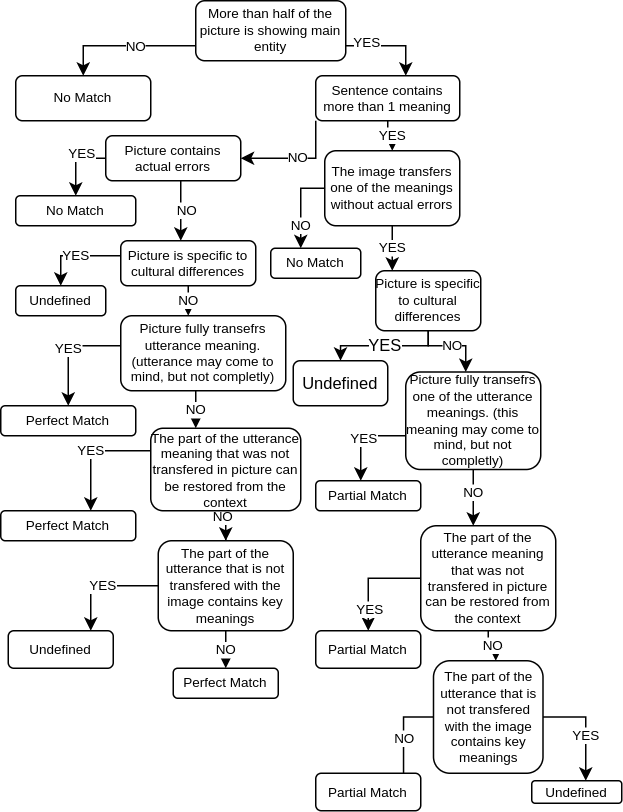
\includegraphics[scale=0.5]{method3.png}
\caption{Labeling Methodology}
\label{LabelingMethod}
\end{figure}
